\documentclass{beamer}
\mode<presentation>
\usepackage{amsmath}
\usepackage{amssymb}
\usepackage{bm}


%\usepackage{advdate}
\usepackage{adjustbox}
\usepackage{subcaption}
%\usepackage{enumitem}
\usepackage{enumerate}
\usepackage{multicol}
\usepackage{mathtools}
\usepackage{listings}
\usepackage{url}
\def\UrlBreaks{\do\/\do-}
\usetheme{Boadilla}
\usecolortheme{lily}
\setbeamertemplate{footline}
{
  \leavevmode%
  \hbox{%
  \begin{beamercolorbox}[wd=\paperwidth,ht=2.25ex,dp=1ex,right]{author in head/foot}%
    \insertframenumber{} / \inserttotalframenumber\hspace*{2ex} 
  \end{beamercolorbox}}%
  \vskip0pt%
}
\setbeamertemplate{navigation symbols}{}

\providecommand{\nCr}[2]{\,^{#1}C_{#2}} % nCr
\providecommand{\nPr}[2]{\,^{#1}P_{#2}} % nPr
\providecommand{\mbf}{\mathbf}
\providecommand{\pr}[1]{\ensuremath{\Pr\left(#1\right)}}
\providecommand{\qfunc}[1]{\ensuremath{Q\left(#1\right)}}
\providecommand{\sbrak}[1]{\ensuremath{{}\left[#1\right]}}
\providecommand{\lsbrak}[1]{\ensuremath{{}\left[#1\right.}}
\providecommand{\rsbrak}[1]{\ensuremath{{}\left.#1\right]}}
\providecommand{\brak}[1]{\ensuremath{\left(#1\right)}}
\providecommand{\lbrak}[1]{\ensuremath{\left(#1\right.}}
\providecommand{\rbrak}[1]{\ensuremath{\left.#1\right)}}
\providecommand{\cbrak}[1]{\ensuremath{\left\{#1\right\}}}
\providecommand{\lcbrak}[1]{\ensuremath{\left\{#1\right.}}
\providecommand{\rcbrak}[1]{\ensuremath{\left.#1\right\}}}
\providecommand{\rank}{\text{rank}}
\theoremstyle{remark}
\newtheorem{rem}{Remark}
\newcommand{\sgn}{\mathop{\mathrm{sgn}}}
\providecommand{\abs}[1]{\left\vert#1\right\vert}
\providecommand{\res}[1]{\Res\displaylimits_{#1}} 
\providecommand{\norm}[1]{\lVert#1\rVert}
\providecommand{\mtx}[1]{\mathbf{#1}}
\providecommand{\mean}[1]{E\left[ #1 \right]}
\providecommand{\fourier}{\overset{\mathcal{F}}{ \rightleftharpoons}}
%\providecommand{\hilbert}{\overset{\mathcal{H}}{ \rightleftharpoons}}
\providecommand{\system}{\overset{\mathcal{H}}{ \longleftrightarrow}}
	%\newcommand{\solution}[2]{\vec{Solution:}{#1}}
%\newcommand{\solution}{\noindent \vec{Solution: }}
\providecommand{\dec}[2]{\ensuremath{\overset{#1}{\underset{#2}{\gtrless}}}}
\newcommand{\myvec}[1]{\ensuremath{\begin{pmatrix}#1\end{pmatrix}}}
\newenvironment{amatrix}[1]{%
  \left(\begin{array}{@{}*{#1}{c}|c@{}}
}{%
  \end{array}\right)
}
\let\vec\mathbf

\lstset{
%language=C,
frame=single, 
breaklines=true,
columns=fullflexible
}

%\numberwithin{equation}{section}

\title{Matgeo-2.10.28}
\author{Harichandana Varanasi-ai25btech11039}

\date{\today} 
\begin{document}

\begin{frame}
\titlepage
\end{frame}

\section*{Outline}

\begin{frame}
\frametitle{Question}
% Q2 (2.7.11)
\textbf{Q 2.10.28.}
For non-zero vectors $\vec a,\vec b,\vec c$, the relation
\[
\bigl|(\vec a\times \vec b)\cdot \vec c\bigr|=\|\vec a\|\,\|\vec b\|\,\|\vec c\|
\]
holds if and only if
\begin{enumerate}
  \item $\vec a\cdot\vec b=0,\; \vec b\cdot\vec c=0$
  \item $\vec b\cdot\vec c=0,\; \vec c\cdot\vec a=0$
  \item $\vec c\cdot\vec a=0,\; \vec a\cdot\vec b=0$
  \item $\vec a\cdot\vec b=\vec b\cdot\vec c=\vec c\cdot\vec a=0$
\end{enumerate}


\end{frame}
%
\begin{frame}

\begin{solution}
Let
\begin{align}
A=\myvec{\vec{a}&\vec{b}&\vec{c}},\qquad 
G=A^\top A
=\myvec{
\vec{a}^\top\vec{a} & \vec{a}^\top\vec{b} & \vec{a}^\top\vec{c}\\
\vec{b}^\top\vec{a} & \vec{b}^\top\vec{b} & \vec{b}^\top\vec{c}\\
\vec{c}^\top\vec{a} & \vec{c}^\top\vec{b} & \vec{c}^\top\vec{c}}
\label{eq:gram-matrix}
\end{align}
be the column and Gram matrices of $\vec{a},\vec{b},\vec{c}$.
The given magnitude equals $\abs{\det A}$, so
\begin{align}
\abs{\det A}^{\,2}=(\det A)^2
=\det\!\paren{A^\top A}
=\det G .
\label{eq:det-square}
\end{align}
By Hadamard’s inequality for the positive semidefinite matrix $G$,
\begin{align}
\det G
\le (\vec{a}^\top\vec{a})\,
   (\vec{b}^\top\vec{b})\,
   (\vec{c}^\top\vec{c})
= \|\vec{a}\|^{2}\,\|\vec{b}\|^{2}\,\|\vec{c}\|^{2},
\label{eq:hadamard-bound}
\end{align}
with equality \emph{iff} $G$ is diagonal, i.e., the columns of $A$ are pairwise orthogonal:
\begin{align}
\vec{a}^\top\vec{b}=0,\qquad
\vec{b}^\top\vec{c}=0,\qquad
\vec{c}^\top\vec{a}=0 .
\label{eq:orth}
\end{align}
\end{solution}
\end{frame}
\begin{frame}{Solution}
    \begin{solution}

Taking square roots in 4.2 and 4.3 yields
\begin{align}
\abs{\det A}
= \|\vec{a}\|\,\|\vec{b}\|\,\|\vec{c}\|
\iff
4.4 holds.
\label{eq:final}
\end{align}
Hence, the correct option is \(\boxed{\text{(d)}}\).
\end{solution}
\end{frame}
\begin{frame}{Plot}
     \begin{figure}[h!]
\centering
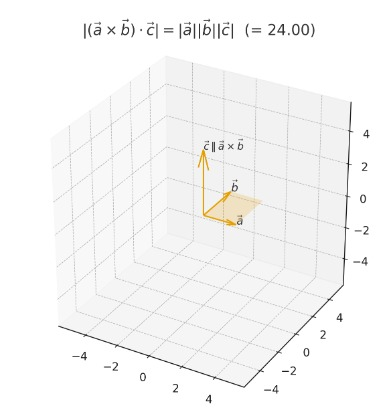
\includegraphics[width=0.5\linewidth]{figs/2.10.28.jpeg}
\caption{Illustration of $|( \vec a\times\vec b)\cdot\vec c|=|\vec a|\,|\vec b|\,|\vec c|$ with $\vec a\perp\vec b$ and $\vec c\parallel(\vec a\times\vec b)$.}


\end{figure}
\end{frame}

\end{document}
